\begin{figure}[H]
	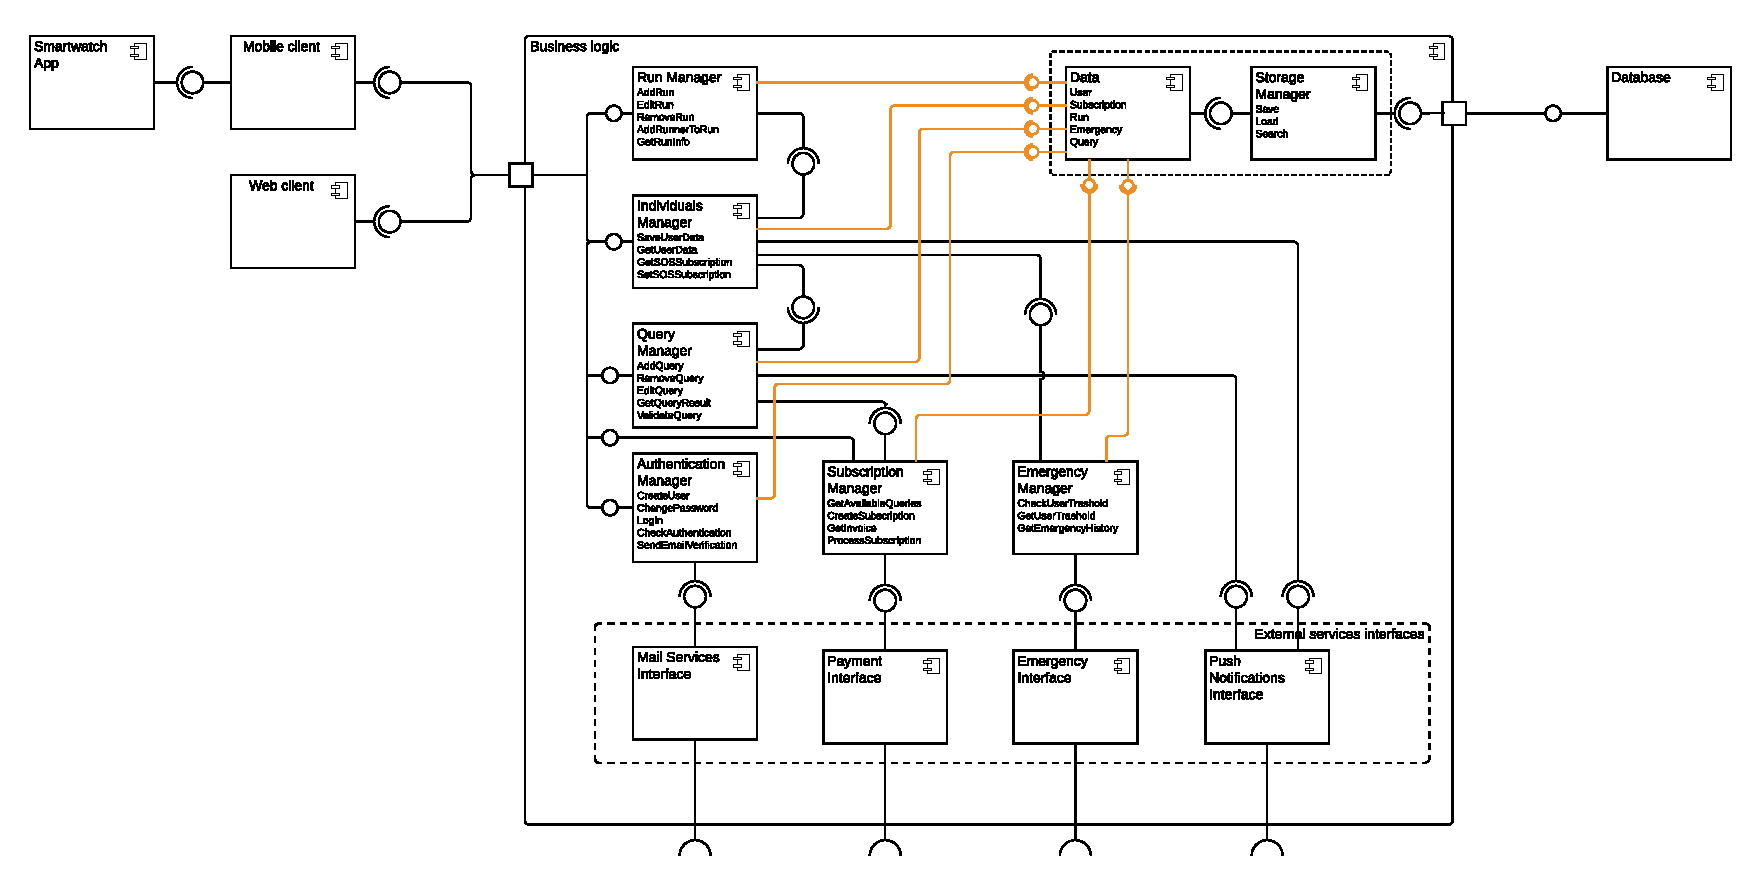
\includegraphics[width=\textwidth,height=\textheight,keepaspectratio]{assets/ComponentDiagram.pdf}
	\caption{Component Diagram}
	\label{fig:CD}
\end{figure}


\noindent The picture shows the components of the application divided in Client, Business Logic and Data.

Below are described more in detail all the components and interfaces that the system uses to offer its functionalities.

\paragraph{Smartwatch device} \mbox{} \newline
The Smartwatch device is directly connected to the mobile app of the user and is not required to interact with the business logic.
Data coming from the sensors of the smartwatch are sent to the mobile app via bluetooth.

\paragraph{Mobile client and Web client} \mbox{} \newline
The clients of the system, 
Mobile client is used by individuals that want to exploit the services of Data4Help.

\paragraph{Individuals Manager} \mbox{} \newline
The Individuals manager has to 
\begin{itemize}
    \item notify the database when there are new data available and store them into it;
    \item manage user requests for old health parameters, accessing Data4help database;
    \item ask the user if agrees to be monitored by a company that has requested an individual query, sending him a push notification;
    \item communicate data to Emergency manager (only if user is subscribed to AutomatedSOS);
\end{itemize}


\paragraph{Authentication Manager} \mbox{} \newline
The component that manages users log-in and registration and is in charge of:
\begin{itemize}
    \item permitting user login
    \item changing user authentication information
    \item adding new user to database
    \item interfacing with Email interface in order to send email verifications
\end{itemize}
information of the users.
\begin{itemize}
    \item \textbf{Companies}
    In case of companies, the Login manager stores email;
    \item \textbf{Individuals}
    In case of individuals, the Login manager stores email, password and a Fiscal Code/Social Security Number.
\end{itemize}

\paragraph{Query Manager} \mbox{} \newline
The core component of the Business unit. It is in charge of:
\begin{itemize}
    \item \textbf{Get query results};
    \item \textbf{Validating queries}: verify if there are the correct number of users involved in the scope of the query (in case of a query on group of individuals), and if a company is allowed to do a query according to its payment subscription;
    \item \textbf{Adding queries} to a company account;
    \item \textbf{Deleting queries} from a company account that wish to unsubscribe from a monthly query;
    \item \textbf{Updating queries}, when a company has subscribed to a query and wants to edit its query; interacts with the Push Notification interface to send the "New data" notification.
\end{itemize}

\paragraph{Subscription Manager} \mbox{} \newline
The component is in charge of managing the subscription of companies to a payment plan offered by Data4Help.
It has to:
\begin{itemize}
    \item \textbf{Subscribe}: let companies subscribe to new payment plans;
    \item \textbf{Store} in the database subscriptions of every company and the eventual query left;
    \item \textbf{Let companies see} their subscription detail;
    \item \textbf{Send companies} their monthly invoice.
\end{itemize}



\paragraph{Emergency Manager} 
\mbox{} \newline
The component is in charge of 
\begin{itemize}
    \item \textbf{evaluating} user health parameters;
    \item \textbf{store} in the database threshold parameters for users subscribed to AutomatedSOS;
    \item \textbf{checking} when a parameter of a user goes below the threshold. If so, the component is in charge to communicate with ambulance API throughout the Emergency interface.
\end{itemize}


\paragraph{Run Manager} \mbox{} \newline
The component is in charge of:
\begin{itemize}
    \item \textbf{Creating}: allows user organizers to create new races;
    \item \textbf{Listing run}: let a list of runs be available to users;
    \item \textbf{Adding} new runners to a race;
    \item \textbf{Managing}: let run organizers manage a race's information.
\end{itemize}


\paragraph{External services interface} \mbox{} \newline
The system is provided with 3 interfaces components that are in charge of communicating with the external services API.
The interfaces are:
\begin{itemize}
    \item Push Notification Interface: communicates with a push notification server API;
    \item Emergency Services Interface: communicates with Ambulance API provided by Hospitals;
    \item Mail Services Interface: communicates with email SMTP server.
\end{itemize}


\paragraph{} \mbox{} \newline

